\iffalse
\let\negmedspace\undefined
\let\negthickspace\undefined
\documentclass[journal,12pt,twocolumn]{IEEEtran}
\usepackage{cite}
\usepackage{amsmath,amssymb,amsfonts,amsthm}
\usepackage{algorithmic}
\usepackage{graphicx}
\usepackage{textcomp}
\usepackage{xcolor}
\usepackage{txfonts}
\usepackage{listings}
\usepackage{enumitem}
\usepackage{mathtools}
\usepackage{gensymb}
\usepackage{comment}
\usepackage[breaklinks=true]{hyperref}
\usepackage{tkz-euclide} 
\usepackage{listings}
\usepackage{gvv}                                        
\def\inputGnumericTable{}                                 
\usepackage[latin1]{inputenc}                                
\usepackage{color}                                            
\usepackage{array}                                            
\usepackage{longtable}                                       
\usepackage{calc}                                             
\usepackage{multirow}                                         
\usepackage{hhline}                                           
\usepackage{ifthen}                                           
\usepackage{lscape}
\newtheorem{theorem}{Theorem}[section]
\newtheorem{problem}{Problem}
\newtheorem{proposition}{Proposition}[section]
\newtheorem{lemma}{Lemma}[section]
\newtheorem{corollary}[theorem]{Corollary}
\newtheorem{example}{Example}[section]
\newtheorem{definition}[problem]{Definition}
\newcommand{\BEQA}{\begin{eqnarray}}
\newcommand{\EEQA}{\end{eqnarray}}
\newcommand{\define}{\stackrel{\triangle}{=}}
\theoremstyle{remark}
\newtheorem{rem}{Remark}
\begin{document}

\bibliographystyle{IEEEtran}
\vspace{3cm}

\title{GATE: XE - 76.2022}
\author{EE23BTECH11224 - Sri Krishna Prabhas Yadla$^{*}$% <-this % stops a space
}
\maketitle
\newpage
\bigskip

\renewcommand{\thefigure}{\arabic{figure}}
\renewcommand{\thetable}{\arabic{table}}


\vspace{3cm}
\textbf{Question:} A spring-mass system having a mass $m$ and spring constant $k$, placed horizontally on a foundation, is connected to a vertically hanging mass $m$ with the help of an inextensible string. Ignore the friction in the pulleys and also the inertia of pulleys, string and spring. Gravity is acting vertically downward as shown. The natural frequency of the system in rad/s is 
\begin{figure}[htbp]
	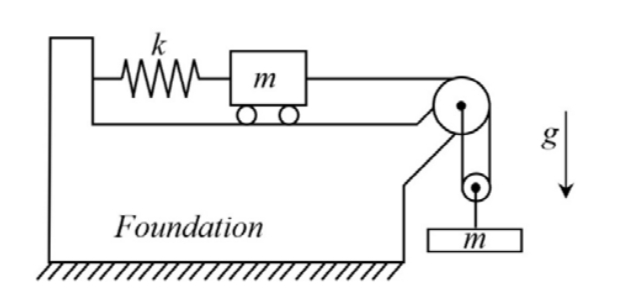
\includegraphics[width=\columnwidth]{2022/XE/76/figs/question_xe76_22.jpg}
	\label{fig:question_xe76_22}
\end{figure}
\begin{enumerate}[label=(\Alph*)]
\item $\sqrt{\frac{4k}{3m}}$
\item $\sqrt{\frac{k}{2m}}$
\item $\sqrt{\frac{k}{3m}}$
\item $\sqrt{\frac{4k}{5m}}$
\end{enumerate}
\hfill(GATE XE 2022)
\\
\solution
\fi
\begin{table}[htbp]
	\centering
	\def\arraystretch{1.5}
	\begin{tabular}{|c|p{4cm}|p{1.5cm}|}
\hline
\textbf{Parameters} & \textbf{Description} & \textbf{Value} \\
\hline
$x(t)$ & Displacement of mass $m$ on foundation at time $t$ & \\
\hline
$x(0)$ & Displacement of mass $m$ on foundation at time $t=0$ & 0 \\
\hline
$x'(0)$ & Velocity of mass $m$ on foundation at time $t=0$ & 0\\
\hline
\end{tabular}

	\caption{Parameters}
	\label{tab:parameters_xe76}
\end{table}
\begin{align}
T-kx &= m\frac{d^2x}{dt^2} \\
mg - 2T &= m\frac{d^2\brak{\frac{x}{2}}}{dt^2} \\
\implies mg - 2kx &= \frac{5}{2}m\frac{d^2x}{dt^2}\\
\label{xe76_L(x'')}\frac{d^2x}{dt^2} &\system{L} s^2X(s)-sx(0)-x'(0) \\
\label{xe76_L(t^n)}t^n &\system{L} \frac{n!}{s^{n+1}}
\end{align}
From the Laplace transforms \eqref{xe76_L(x'')} and \eqref{xe76_L(t^n)}, we get
\begin{align}
\frac{mg}{s}-2kX(s)&=\frac{5}{2}m\brak{s^2X(s)-sx(0)-x'(0)}\\
\implies X(s) &= \frac{\frac{2g}{5}}{s\brak{s^2+\frac{4k}{5m}}}\\
&= \frac{mg}{2ks}-\frac{mgs}{2k\brak{s^2+\frac{4k}{5m}}}\\
\label{xe76_L(cos{at})} \cos{at} &\system{L} \frac{s}{s^2+a^2}
\end{align}
From the Laplace transforms \eqref{xe76_L(t^n)} and \eqref{xe76_L(cos{at})}, we get
\begin{align}
x(t) &= \frac{mg}{2k}\brak{1-\cos{\brak{\sqrt{\frac{4k}{5m}}t}}}u(t)\\
\implies \omega &= \sqrt{\frac{4k}{5m}}
\end{align}
\begin{figure}[htbp]
	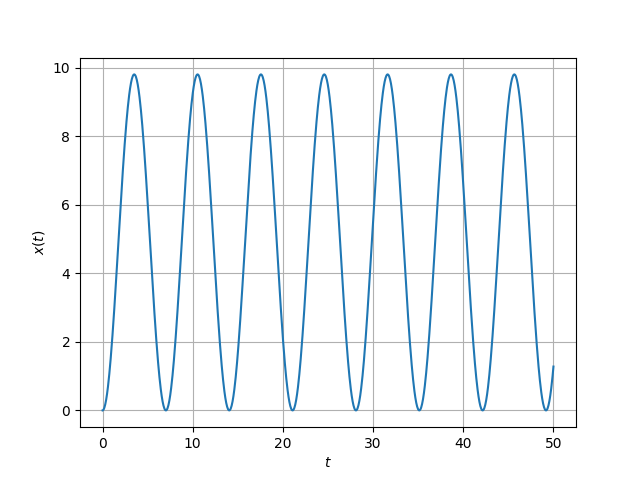
\includegraphics[width=\columnwidth]{2022/XE/76/figs/plot.png}
	\caption{Plot of $x(t)$ for $m=1kg$, $k=1N/m^2$}
	\label{fig:plot_xe76}
\end{figure}
